\subsubsection{Database}

\par Il diagramma E-R (entità-relazione) riportato a seguito illustra la struttura e le relazioni all'interno del database.

\begin{figure}[H]
    \centering
    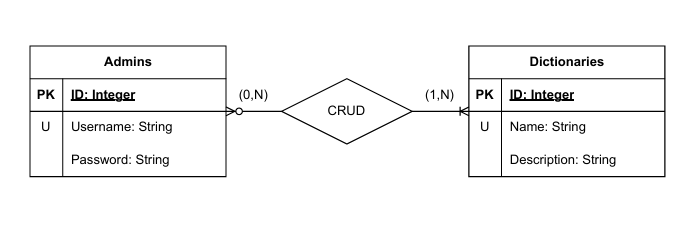
\includegraphics[width=0.95\textwidth]{assets/Database/DiagrammiDB.png}
    \caption{Diagramma E-R dell'interazione tra Admins (Tecnici) e \glossario{dizionari dati} per le operazioni \glossario{CRUD}}
\end{figure}

\subsubsection{Descrizione}
\par Il diagramma utilizza la notazione standard per le descrizioni dei database relazionali; le entità sono rappresentate da rettangoli, mentre le relazioni sono le linee che collegano le entità. All'interno del diagramma sono presenti le seguenti sigle:
\begin{itemize}
    \item \textbf{PK}: chiave primaria;
    \item \textbf{U}: attributi, o campi, della tabella.
\end{itemize}

\par Le linee terminano con dei simboli che ne indicano la cardinalità. Le tabelle sono inoltre collegate a un rombo che rappresenta la relazione tra di esse: questa relazione non è una tabella, ma serve solo a scopo illustrativo.

\paragraph{Tabella Admins}
\par La tabella \textbf{Admins} contiene i seguenti campi:
\begin{itemize}
    \item \textbf{PK ID}: un identificatore unico per ogni amministratore, di tipo integer;
    \item \textbf{U Username}: il nome utente dell'amministratore, di tipo string;
    \item \textbf{Password}: la password dell'amministratore, di tipo string.
\end{itemize}
\par Ogni entry della tabella descrive un Admin, cioè un Tecnico che può eseguire operazioni \glossario{CRUD} sui dizionari dati.

\paragraph{Tabella Dictionaries}
\par La tabella \textbf{Dictionaries} include i seguenti campi:
\begin{itemize}
    \item \textbf{PK ID}: un identificatore unico per ogni dizionario, di tipo integer;
    \item \textbf{U Name}: il nome del dizionario, di tipo string;
    \item \textbf{Description}: la descrizione del dizionario, di tipo string.
\end{itemize}

\paragraph{Relazione}
Il diagramma mostra anche le operazioni CRUD (Create, Read, Update, Delete), ossia le interazioni tra i Tecnici e i \glossario{dizionari dati}.

\begin{itemize}
      \item Relazione \textbf{0-N}: un admin può eseguire operazioni CRUD su 0 o N dizionari;
    \item Relazione \textbf{1-N} : un dizionario dati può essere gestito da 1 o N admin.
\end{itemize}